\section{算子方程的稳定性}
\label{sec:opeq-stability}

前两节回答了解是否存在、是否唯一。实际数据总带有误差，即使方程对精确数据有唯一解，也还要问：数据改变一点，解会不会改变很多？这个问题只有在固定了输入和输出的范数之后才有确切含义，因为“一点”和“很多”都要用范数来量。本节先把三个要求并列写出，再分别考察第一类方程中的小奇异值和第二类方程中的共振参数。

\paragraph{适定问题}
设$X,Y$是赋范空间，$A:X\to Y$是有界线性算子，考虑方程$Ax=y$。按Hadamard的说法，若同时满足
\begin{enumerate}
  \item 存在：对每个$y\in Y$都有解；
  \item 唯一：解至多一个；
  \item 稳定：解连续依赖于数据，即$A^{-1}:Y\to X$连续，
\end{enumerate}
就称这个方程是\term{适定问题}（well-posed problem），否则称为\term{不适定问题}（ill-posed problem）。

三条要求相互独立，也都依赖于所取的范数。同一个求导问题，若把数据空间的范数加强到包含导数，误差放大就可能消失；所以说一个方程“不稳定”时，必须同时说明在哪对范数之下。$X,Y$都是Banach空间时，前两条已经蕴含第三条：有界双射的逆有界，这正是第~\ref{chap:linear-operators}章开映射定理的推论。因此在完备空间中，失去稳定性总是伴随着失去存在性，即像不是整个空间，甚至不闭。

\paragraph{趋于零的奇异值}
设$K:H_1\to H_2$为紧算子，并有无限多个正奇异值，$\sigma_j\to0$。在最小范数解的意义下，即使限制在可解的数据上，解也不连续依赖于数据。取数据扰动$\delta g_j=\sigma_ju_j$，则$\lVert\delta g_j\rVert=\sigma_j\to0$；它满足Picard条件，相应的最小范数解扰动为
\[
  \delta f_j=\frac{\langle u_j,\delta g_j\rangle}{\sigma_j}v_j=v_j,\qquad\lVert\delta f_j\rVert=1 .
\]
数据误差趋于零，解的误差却始终为$1$。所以映射$g\mapsto f^\dagger$在$\operatorname{Ran}K$上是无界的线性映射。

只有有限多个正奇异值时情况相反：Picard级数中各项都除以不小于$\sigma_{\min}$的数，所以$\lVert f^\dagger\rVert\leq\lVert g\rVert/\sigma_{\min}$，其中$\sigma_{\min}$是最小的正奇异值。秩二例子中$\sigma_{\min}=1/3$，误差至多放大三倍。误差放大的程度不由“算子是否可逆”这一定性性质决定，而由奇异值离零有多远决定。

\begin{theorem}[紧算子的像不闭]
\label{thm:opeq-compact-range}
设$K:H_1\to H_2$为紧算子，$\operatorname{Ran}K$是无限维的。则$\operatorname{Ran}K$在$H_2$中不闭，$K$限制在$(\ker K)^\perp$上的逆$\operatorname{Ran}K\to(\ker K)^\perp$无界。
\end{theorem}

\begin{proof}
先证逆无界。设逆有界，范数为$c$，则$\operatorname{Ran}K$中范数不超过$1$的元素都是$K$作用在$(\ker K)^\perp$中范数不超过$c$的元素上的像。$K$紧，这些像组成相对紧集，所以$\operatorname{Ran}K$中的每个有界序列都有在$H_2$中收敛的子列。但$\operatorname{Ran}K$是无限维子空间，由Gram--Schmidt过程可以在其中取一列标准正交向量，它们两两距离都是$\sqrt2$，没有收敛子列；这正是第~\ref{chap:functions-as-vectors}章所说的无限维闭球不紧。矛盾，所以逆无界。

再证像不闭。若$\operatorname{Ran}K$闭，它作为闭子空间是Hilbert空间，$K$限制在闭子空间$(\ker K)^\perp$上就是两个Hilbert空间之间的有界双射。由开映射定理，其逆有界，与上一段矛盾。
\end{proof}

结合上一节，无限秩紧算子的第一类方程三条要求全部失效：像不闭，存在性只对一个稠密而不闭的子空间成立；零空间可能非零；在像上解也不连续依赖于数据。对第一类方程，这种不适定不是例外情形，而是无限维紧算子的一般性质。

\paragraph{累积积分的误差放大}
对累积积分$V$，奇异值$\sigma_k=1/((k-\frac12)\pi)$按$1/k$衰减。取真解$f=1$，精确数据$g=Vf=x$。在数据上加入扰动$\delta u_{20}$，$\delta=0.01$，最小范数解多出$(\delta/\sigma_{20})v_{20}$，其范数为$19.5\pi\delta\approx0.61$，振幅$\sqrt2\times0.61\approx0.87$。图~\ref{fig:opeq-noise-amplification}中两条数据曲线几乎重合，解中却出现明显的快速振荡。

\begin{figure}[!htb]
  \centering
  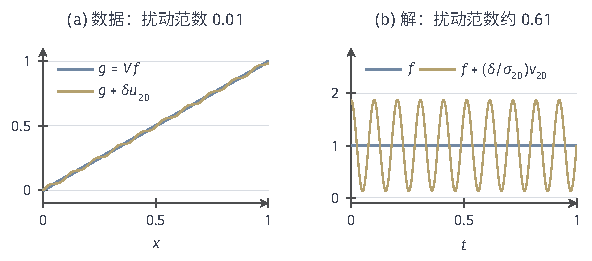
\includegraphics[width=100.2mm]{figures/02-abstract-mathematics/03-function-spaces/tikz/c3-noise-amplification/figure.pdf}
  \caption{第一类方程$Vf=g$（$(Vf)(x)=\int_0^xf$）中小奇异值放大扰动。真解$f=1$，数据$g=x$。(a)数据加上范数为$0.01$的扰动$\delta u_{20}$，与原数据几乎重合。(b)相应的最小范数解多出$(\delta/\sigma_{20})v_{20}$，振幅约$0.87$、范数约$0.61$，放大倍数$1/\sigma_{20}=19.5\pi\approx61$。}
  \label{fig:opeq-noise-amplification}
\end{figure}

这一机制与上一节“求解$Vf=g$就是求导”的结论是同一件事。$V$把快速振荡的输入平均掉，反解时必须把同样的振荡放大回去，振荡越快，放大倍数$1/\sigma_k=(k-\frac12)\pi$越大。求导在$L^2$范数下不连续：$\sin(n\pi x)/n$的范数趋于零，导数$\pi\cos(n\pi x)$的范数却不趋于零。

\paragraph{有限截断与误差的两部分}
一个自然的做法是只保留前$m$个奇异方向，令
\[
  f_m^\delta=\sum_{j\leq m}\frac{\langle u_j,g^\delta\rangle}{\sigma_j}v_j ,
\]
其中$g^\delta$是带误差的数据，$\lVert g^\delta-g\rVert\leq\delta$，$g=Kf^\dagger$为精确数据。这个截断算子有界，范数为$1/\sigma_m$。设$f_m$是用精确数据得到的截断解，则$f_m^\delta-f^\dagger=(f_m-f^\dagger)+(f_m^\delta-f_m)$。第一项是舍弃方向上的系数，第二项只含前$m$个方向上数据误差的放大；由Bessel不等式，
\begin{equation}
  \lVert f_m^\delta-f^\dagger\rVert\leq\Bigl(\sum_{j>m}\lvert\langle v_j,f^\dagger\rangle\rvert^2\Bigr)^{1/2}+\frac{\delta}{\sigma_m}.
  \label{eq:opeq-truncation-split}
\end{equation}

式~\eqref{eq:opeq-truncation-split}中，$m$增大使第一项减小、第二项增大。固定$m$时得到的是有界算子，所以截断本身是稳定的；但它求的不再是原方程的精确解，而且稳定常数$1/\sigma_m$随$m$变坏。因此不能从形式逆或某个有限截断直接推出可靠恢复：截断位置必须结合误差水平$\delta$和真解在高阶方向上的大小来选。这种选择以及用惩罚项代替硬截断的方法，属于正则化问题，可参考\BookChapterRef{chap:function-fitting-regularization}{卷五第10章“函数拟合与正则化”}；有限维中奇异值截断与条件数的关系，可参考\BookChapterRef{chap:solution-error-regularization}{卷二第14章“求解误差、正则化与方法选择”}。

\paragraph{第二类方程与共振参数}
第二类方程在$1/\lambda$不是特征值时有有界逆，因而是适定的。但“有界”并不说明界有多大。设$K$紧自伴，$\lambda$不是任何$1/\lambda_j$。由上一节的方向表示，$(I-\lambda K)^{-1}$在零空间上乘以$1$，在第$j$个特征方向上乘以$1/(1-\lambda\lambda_j)$，所以
\[
  \bigl\lVert(I-\lambda K)^{-1}\bigr\rVert=\max\Bigl\{\sup_j\frac{1}{\lvert1-\lambda\lambda_j\rvert},\ 1\Bigr\},
\]
其中$1$来自零空间上的恒等作用。$H$无限维而零空间为$\{0\}$时，特征值有无穷多个且趋于零，相应乘子的倒数趋于$1$，所以这一项不改变结果。$\lambda$靠近某个$1/\lambda_k$时，相应乘子的倒数趋于无穷，数据在$e_k$方向上的误差被放大$1/\lvert1-\lambda\lambda_k\rvert$倍。

秩二例子中，$\lVert(I-\lambda T)^{-1}\rVert=\max\{1/\lvert1-\lambda\rvert,1/\lvert1-\lambda/3\rvert,1\}$。$\lambda=0.99$时这个范数为$100$：源项在常数方向上$10^{-3}$的误差，会使解在同一方向上改变$0.1$，而其他方向上的误差几乎不被放大。与第一类方程比较，第二类方程的敏感性集中在共振参数附近的有限个方向上，远离这些参数时有统一的界；第一类方程的敏感性则来自无穷多个趋于零的奇异值，任何参数都无法消除。

\paragraph{算子的扰动}
实际计算中，算子本身也常被近似，例如用有限秩核代替原来的积分核。Neumann级数给出这时的稳定性判据。设$B=I-\lambda K$有有界逆，$E$是有界算子，且$\lVert B^{-1}\rVert\lVert E\rVert<1$。写成$B+E=B(I+B^{-1}E)$，由定理~\ref{thm:opeq-neumann}，$I+B^{-1}E$可逆，于是$B+E$可逆且
\[
  \bigl\lVert(B+E)^{-1}\bigr\rVert\leq\frac{\lVert B^{-1}\rVert}{1-\lVert B^{-1}\rVert\lVert E\rVert}.
\]
若$K_m$是$K$的有限秩近似，取$E=-\lambda(K_m-K)$，只要$\lvert\lambda\rvert\lVert K-K_m\rVert\lVert B^{-1}\rVert<1$，近似方程就仍然唯一可解，并有可控的稳定常数。这一条件同时依赖近似误差和$\lVert B^{-1}\rVert$：参数越靠近共振值，对算子近似的精度要求越高。

对第一类方程，同样的论证无法进行，因为$K$本身没有有界逆可以作为起点。这再次说明两类方程的区别来自恒等项的结构：恒等项提供了一个可逆的主部，紧算子只是对它的扰动；第一类方程中紧算子就是全部，它的逆的不连续性无法通过细化近似消除。
